% y = arth(x)
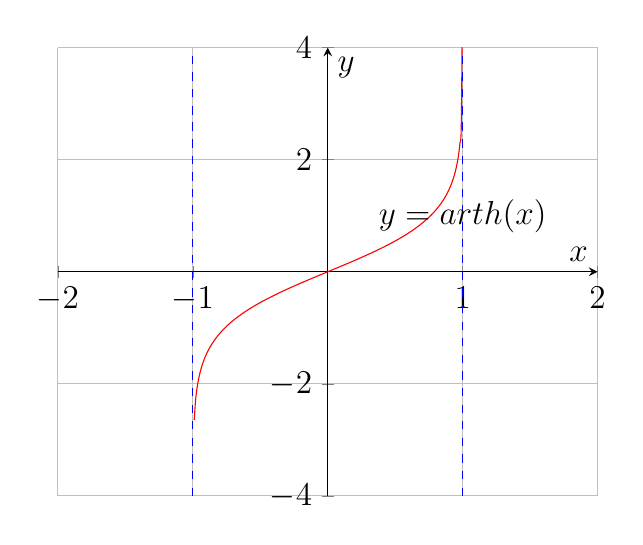
\begin{tikzpicture}
  \begin{axis}[xmin=-2,xmax=2,ymin=-4,ymax=4, grid=both, font=\large, axis lines=middle, smooth, xlabel={$x$}, ylabel={$y$}]
    \addplot[draw=red,domain=-1:1,samples=200] {(1/2)*ln((1 + x)/(1 - x))};
    \addplot[dashed, draw=blue, mark=none] coordinates {(1, -4) (1, 4)};
    \addplot[dashed, draw=blue, mark=none] coordinates {(-1, -4) (-1, 4)};
    \node at (axis cs:1,1) {$y = arth(x)$};
  \end{axis}
\end{tikzpicture}
